\documentclass[a4paper,ngerman,11pt,bibtotoc]{scrartcl}

\usepackage[utf8]{inputenc}

\usepackage[ngerman]{babel}

\usepackage{amsmath, amsthm, amssymb, stmaryrd, color, graphicx, mathtools, mathrsfs}
\usepackage{setspace}
\usepackage{bussproofs}
\usepackage{array}
\usepackage{booktabs}
\usepackage{comment}
\usepackage{textcomp}
\usepackage{stmaryrd}

\usepackage{tikz}
\usetikzlibrary{shapes,arrows}

\usepackage[protrusion=true,expansion=true]{microtype}

\usepackage{lmodern}
\usepackage{tabto}

\usepackage[backend=bibtex,style=alphabetic]{biblatex}
\usepackage[babel]{csquotes}
\bibliography{literatur}

\usepackage{titling}

\usepackage[all]{xy}

\usepackage[colorlinks=true, linkcolor=blue, urlcolor=blue, citecolor=blue]{hyperref}
\usepackage{cleveref}			% Referenzen mit Name

\usepackage{icomma}				% Korrektes Typesetting von Kommazahlen


\usepackage{algorithm}
\usepackage{algpseudocode}
\algrenewcommand{\algorithmiccomment}[1]{\hskip3em$\slash\slash$ #1}
\newcommand{\LineFor}[2]{\State\algorithmicfor\ {#1}\ \algorithmicdo\ {#2} \algorithmicend\ \algorithmicfor}

\usepackage{listings}			% Anzeige von Sourcecode


\setlength\parskip{\medskipamount}
\setlength\parindent{0pt}

\theoremstyle{definition}
\newtheorem{defn}{Definition}[section]
\newtheorem{axiom}[defn]{Axiom}
\newtheorem{bsp}[defn]{Beispiel}

\theoremstyle{plain}

\newtheorem{prop}[defn]{Proposition}
\newtheorem{motto}[defn]{Motto}
\newtheorem{ueberlegung}[defn]{Überlegung}
\newtheorem{lemma}[defn]{Lemma}
\newtheorem{kor}[defn]{Korollar}
\newtheorem{hilfsaussage}[defn]{Hilfsaussage}
\newtheorem{satz}[defn]{Satz}

\theoremstyle{remark}
\newtheorem{erin}[defn]{Erinnerung}
\newtheorem{bem}[defn]{Bemerkung}
\newtheorem{beob}[defn]{Beobachtung}
\newtheorem{aufg}[defn]{Aufgabe}

\clubpenalty=10000
\widowpenalty=10000
\displaywidowpenalty=10000

\newcommand{\IZ}{\mathbb{Z}}
\newcommand{\IQ}{\mathbb{Q}}
\newcommand{\IR}{\mathbb{R}}
\newcommand{\IC}{\mathbb{C}}
\newcommand{\IN}{\mathbb{N}}
\newcommand{\Ic}{\mathcal{I}}
\newcommand{\Jc}{\mathcal{J}}
\newcommand{\Hc}{\mathcal{H}}
\newcommand{\Tc}{\mathcal{T}}
\newcommand{\Sc}{\mathcal{S}}
\newcommand{\Oc}{\mathcal{O}}

\newcommand{\ceil}[1]{\left\lceil#1\right\rceil}

% Nur für dieses Dokument %%%%%%%%%%%%%%%%%%%%%%%%%%%%%%%%%%%%%%

\newcommand{\ClientSet}{\mathscr{C}}
\newcommand{\FacilitySet}{\mathscr{F}}
\newcommand{\allTours}{\mathscr{T}}

\newcommand{\OPT}{OPT}
\newcommand{\CLR}{CLR}
\newcommand{\CLRHFC}{CLRhFC}
\newcommand{\MST}{MST}
\newcommand{\ULF}{ULF}

% C++ from http://tex.stackexchange.com/a/4304
\def\Cpp{{C\nolinebreak[4]\hspace{-.05em}\raisebox{.4ex}{\tiny\bf ++}}}

% Switch between equationsnumbers on the left and on the right (from http://tex.stackexchange.com/a/193538 )
\makeatletter
\newcommand{\leqnomode}{\tagsleft@true}
\newcommand{\reqnomode}{\tagsleft@false}
\makeatother

\renewcommand*\theenumi{\alph{enumi}}
\renewcommand{\labelenumi}{(\theenumi)}

% Set lagnuage and other options for Code snippets
\lstset{language=C++}
\lstset{tabsize=4}
\lstset{basicstyle=\small\ttfamily}
\lstset{frame=Tb, captionpos=b}
\lstset{xleftmargin=1em, xrightmargin=1em, aboveskip=2\medskipamount}

\setcounter{tocdepth}{2}


\usepackage{todonotes}
\usepackage{tabu}


% DOCUMENT %%%%%%%%%%%%%%%%%%%%%%%%%%%%%%%%%%%%%%%%%%%%%%%%%%%%%

\begin{document}
\author{Lukas Graf}
\date{Letzte Aktualisierung: \today}

\selectlanguage{ngerman}
\thispagestyle{empty}


\begin{titlepage}\center
	\textsc{\LARGE Universität Augsburg}\\[1cm]
	
	\textsc{\Large Institut für Mathematik}\\[1.5cm]
	
	% Title
	{\Large Ausarbeitung \\[1cm]}
	zum Programmierprojekt\\[1cm]
	{\huge Capacitated Location Routing \\ with Hard Facility Capacities}

	\begin{center}
		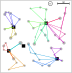
\includegraphics[width=.6\textwidth]{bilder/title.pdf}
	\end{center}		
	
	\vfill
	
	% Author and supervisor
	\begin{minipage}{0.4\textwidth}
		\begin{flushleft} \large
			\emph{von:}\\
			Lukas \textsc{Graf}
		\end{flushleft}
	\end{minipage}
	\begin{minipage}{0.4\textwidth}
		\begin{flushright} \large
			\emph{Betreut von:} \\
			Prof. Dr. Tobias \textsc{Harks}
		\end{flushright}
	\end{minipage}
	
\end{titlepage}

% CONTENT %%%%%%%%%%%%%%%%%%%%%%%%%%%%%%%%%%%%%%%%%%%


\tableofcontents

\newpage
	
\section*{\glqq Abstract\grqq}

\todo[inline]{Zusammenfassung/Überblick der Arbeit}


\section{Capacitated Location Routing (CLR)}

	\subsection{Problemdefinition}

Eine Instanz des \textbf{Capacitated Location Routing Problems (CLR)} ist gegeben durch
\begin{itemize}
	\item einen ungerichteten, zusammenhängenden Graphen $G =(V,E)$,
	\item eine Partition der Knoten in Kunden $\ClientSet$ und Fabrikstandorte $\FacilitySet$,
	\item eine metrischen Kostenfunktion auf den Kanten $c: E \to \IR_{\geq 0}$,
	\item Eröffnungskosten für die Fabriken $\phi: \FacilitySet \to \IR_{\geq 0}$,
	\item Bedarfe der Kunden $d: \ClientSet \to \IR_{\geq 0}$
	\item und eine einheitliche Kapazität $u > 0$ für die Fahrzeuge.		
\end{itemize}
Zulässige Lösungen bestehen aus
\begin{itemize}
	\item einer Teilmenge $F \subseteq \FacilitySet$ von eröffneten Fabriken
	\item und einer Menge von Touren $\Tc = \{T_1, \dots, T_k\}$,
\end{itemize}
sodass gilt:
\begin{itemize}
	\item Zu jeder Tour gibt es eine geöffnete Fabrik $f \in F$, an der diese startet und endet.
	\item Alle Touren zusammen erfüllen alle Bedarfe der Kunden.
	\item Keine der Touren übersteigt die Kapazität $u$.
\end{itemize}
Das Optimierungsziel ist es die Gesamtkosten für das Eröffnen der Fabriken und die gefahrenen Touren zu minimieren, also die Minimierung der Kostenfunktion
\footnote{Wir verwenden hier, dass eine Funktion $\IR$-wertige Funktion $c: M \to \IR$ auf einer Menge $M$ eine Funktion $\tilde{c}: \mathcal{P}(M) \to \IR: M \supseteq N \mapsto \sum_{x \in N} c(x)$ auf der Potenzmenge $\mathcal{P}(M)$ induziert. Zur Vereinfachung der Notation bezeichnen wir diese Funktion dann ebenfalls mit $c$. Unter nochmaliger Anwendung dieser Konvention ließe sich die obige Kostenfunktion daher auch als $c(\Tc) + \phi(F)$ schreiben.}
	\[\sum_{T\in\Tc} c(T) + \sum_{f\in F}\phi(f) \]
	
\begin{beob}
	$\CLR{}$ ist NP-schwer, denn es beinhaltet beispielsweise metrisches TSP (betrachte Instanzen mit $|\FacilitySet| = 1$, $d \equiv 1$ und $u = |\ClientSet|$).
\end{beob}

\begin{bem}
	Gilt $d \equiv 1$ und $u = 1$, so erhält man eine Instanz des (metrischen) \emph{Uncapacitated Facility Location Problems} (\ULF). Statt Touren von den geöffneten Fabriken zu den Kunden zu finden, genügt es hier offensichtlich eine Zuordnung von Kunden zu Fabriken zu bestimmen. Für dieses Problem sind eine ganze Reihe von Approximationsalgorithmen bekannt (vergleiche z.B. \cite{AAfFLP}), unter anderem erweist sich ein einfacher Greedy-Ansatz bereits als $1,861$-approximativ (siehe \cite{GreedyApprox}).
\end{bem}


	\subsection{Ein Approximationsalgorithmus für \CLR}

Der in \cite{AAfCLR} beschriebene $4,38$-approximative\footnote{Die diesem Programmierprojekt zugrunde liegende Implementierung weist allerdings nur eine Approximationsgarantie von $5,722$ auf, da zur approximativen Lösung der \ULF-Instanz ein leichter zu implementierender Greedy-Algorithmus verwendet wurde, anstatt eines anderen Verfahrens mit besserer Approximationsgarantie.} Algorithmus für \CLR basiert im Wesentlichen auf den folgenden Schritten (schematisch dargestellt in \cref{fig:CLRAlg}):
\begin{description}
	\item[\ULF-Phase:] Erstelle eine \ULF-Instanz mit den gleichen Fabriken und Kunden, aber mit um $2/u$ skalierten Kosten. Löse diese Instanz approximativ und eröffne alle hier geöffneten Fabriken auch in der \CLR-Instanz. Es zeigt sich, dass die Kosten einer optimalen Lösung der \ULF-Instanz eine untere Schranke für die optimale Lösung der \CLR-Instanz bildet.
	\item[\MST-Phase:] Ergänze den Graphen der \CLR-Instanz um einen zusätzlichen Knoten $r$ mit kostenlosen Kanten zu allen Fabriken. Erhöhe ferne alle Kanten zwischen Fabriken und Kunden um die halben Eröffnungskosten der jeweiligen Fabrik. Dann finde einen minimalen Spannbaum $B$ in diesem Graphen und öffne in der \CLR-Instanz zusätzlich alle Fabriken, die in $B$ wenigstens einen Kunden als Nachbarn haben. Die Kosten einen solchen Spannbaumes sind erneut eine untere Schranke für die Kosten einer optimalen Lösung der \CLR-Instanz.
	\item[Large Demand-Phase:] Alle Kunden mit Bedarf von mindestens $u$ werden durch $\ceil{d/u}$ Touren mit der jeweils nächsten Fabrik verbunden. Die hierfür anfallenden Anbindungskosten sind höchstens zweimal die entsprechenden Kosten aus der \ULF-Phase.
	\item[Merge-Phase] Betrachte $B$ aus der \MST-Phase als Baum mit Wurzel $r$. Solange dies möglich ist, finde darin einen Teilbaum (mit Wurzel $v$), der einen Gesamtbedarf von mehr als $u$ hat, aber dessen nächstkleinere Teilbäume (beginnend bei den Kindern von $v$) einen Bedarf von höchstens $u$ haben. Ein solcher Baum wird als \emph{Relieve-Tree} bezeichnet.
	 
	Fasse diese kleineren Teilbäume und den \glqq Baum\grqq{} $\{v\}$ so zusammen, dass jede Menge einen Bedarf zwischen $\frac{u}{2}$ und $u$ hat (die letzte ggfls. weniger). Wandle jede der großen Mengen in eine Tour um (durch Verdoppeln der Kanten im entsprechenden Teilbaum und nachfolgendem Abkürzen bei doppelt besuchten Kunden) und verbinde sie mit der nächstliegenden offenen Fabrik. Die Verbindungskosten hierfür sind beschränkt durch das Doppelte der Kosten im Spannbaum $B$ und den entsprechenden Verbindungskosten aus der \ULF-Phase. Die Kunden aus der kleinen Menge bleiben vorerst unversorgt und werden beim nächsten Relieve-Tree neu berücksichtigt.
	
	Ist der verbleibende Gesamtbedarf unter einer Fabrik schließlich kleiner oder gleich $u$, so werden alle im entsprechenden Teilbaum verbliebenen Kunden zu einer Tour (\emph{Remaining-Tour}) zusammengefasst und mit der nächstliegenden offenen Fabrik verbunden. Die Verbindungskosten hierfür sind erneut durch das Doppelte der entsprechenden Kosten aus dem Spannbaum begrenzt.
\end{description}

\begin{figure}[H]
	\begin{tiny}
		
\tikzstyle{Absch} = [rectangle, draw, 
    text centered]
\tikzstyle{keinBeweis} = [rectangle, fill=gray!35, 
    text centered]    

\tikzstyle{BewTeil} = []


\tikzstyle{Box} = [rectangle, draw, 
text centered, rounded corners]
\tikzstyle{Alg} = [rectangle, draw, fill=gray!50, text centered]
\tikzstyle{Text} = [ 
text centered]

\tikzstyle{line} = [draw, -latex']
\tikzstyle{line2} = [draw]


\begin{tikzpicture}[node distance = 5em, auto]

% EINGABE:
\node [Box, text width=20em] (input) {\textbf{Input:} \\ CLR-Instanz $((\ClientSet\cup\FacilitySet,E),c,\phi,d,u)$};
\node [below of=input] (under-input) {};

% ULF-Instanz:
\node [Box, left of=under-input, text width=12em, node distance=7em] (ULF) {\textbf{ULF-Instanz:} \\ $((\ClientSet\cup\FacilitySet,E),c,\phi,d,u)$};
\node [Text, left of=ULF, text width=12em, node distance=15em] (ULF-lower-bound) {$\leadsto$ Untere Schranke: $\OPT(\CLR) \geq \OPT(\ULF)$};
\node [Alg, below of=ULF, text width=12em] (ULF-solving) {löse approximativ (mit Greedy)};

% MST-Instanz:
\node [Box, right of=under-input, text width=12em, node distance=7em] (MST) {\textbf{MST-Instanz:} \\ $((\ClientSet\cup\FacilitySet,E),c,\phi,d,u)$};
\node [Text, right of=MST, text width=12em, node distance=15em] (MST-lower-bound) {$\leadsto$ Untere Schranke: $\OPT(\CLR) \geq \OPT(\MST)$};
\node [Alg, below of=MST, text width=12em] (MST-solving) {löse exakt (mit ???)};

% MERGE-Phase:
\node [Alg, below of=under-input, node distance=10em] (merge) {Merge-Phase:};

\node [Text, below of=merge, node distance=2em] (m-facilities) {Eröffne in $\ULF$ oder $\MST$ verwendete Facilities};

\node [Text, below of=m-facilities, node distance=2em] (m-big-clients) {Verbinde Klienten $v$ mit $d(v)\geq u$ mit nächstliegender offener Fabrik};

\node [Text, below of=m-big-clients, node distance=2em] (m-small-clients) {Für jede durch die $\MST$-Lsg eröffnete Farbik $f$ tue...};

\node [Box, below of=m-small-clients, node distance=10em] (m-relieve) {
	\begin{minipage}{20em}
		\begin{algorithmic}
		\While{$D_f > 0$}
		\State Finde $v \in S_f$ mit $D_v > u$ und f.a. Kinder $w$ von $v$: $D_w \leq u$
		\State Zerlege $S_v$ in Teilbäume ...
		\EndWhile
		\end{algorithmic}
	\end{minipage}
};

\node [Text, below of=m-relieve, node distance=10em] (m-remaining) {Mache rest...};


% AUSGABE:
\node [Box, below of=m-remaining, node distance=4em] (output) {Lösung};

\path [line] (input.south) -- (ULF.north);    
\path [line] (input.south) -- (MST.north); 

\path [line] (ULF-solving.south) -- (merge.north);
\path [line] (MST-solving.south) -- (merge.north);

\path [line] (m-remaining.south) -- (output.north);

\end{tikzpicture}

	\end{tiny}
	\caption{Schematische Darstellung des Algorithmus für CLR}\label{fig:CLRAlg}
\end{figure}

\subsection{Visualisierung des Algorithmus}

Im ersten Teil des Programmierprojektes ging es darum den Ablauf sowie das Ergebnis des oben beschriebenen Algorithmus zu visualisieren. Dazu wurde die existierende Implementierung des Algorithmus um eine Klasse \lstinline|CLR\_Drawing| erweitert. Diese wird zu Beginn des Algorithmus mit der zu lösenden Instanz initialisiert und kann dann an verschiedenen Stellen des Algorithmus aufgerufen werden, um einen Schnappschuss mit dem momentanen Stand zu erstellen. 

\begin{figure}[H]\centering\setlength{\fboxsep}{0pt}
	\fbox{\includegraphics[width=.19\textwidth]{bilder/demo_instance.pdf}}
	\fbox{\includegraphics[width=.19\textwidth]{bilder/demo_ULF.pdf}}
	\fbox{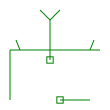
\includegraphics[width=.19\textwidth]{bilder/demo_Tree.pdf}}
	\fbox{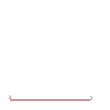
\includegraphics[width=.19\textwidth]{bilder/demo_LargeDemand.pdf}}
	\fbox{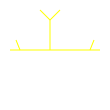
\includegraphics[width=.19\textwidth]{bilder/demo_relieveTree.pdf}}
	
	\fbox{\includegraphics[width=.19\textwidth]{bilder/demo_relieveTour.pdf}}
	\fbox{\includegraphics[width=.19\textwidth]{bilder/demo_remainingTour.pdf}}
	\fbox{\includegraphics[width=.19\textwidth]{bilder/demo_singleTour.pdf}}
	\fbox{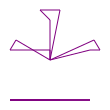
\includegraphics[width=.19\textwidth]{bilder/demo_allTours.pdf}}
	
	\caption{Ausgabe der Klasse \lstinline|CLR\_Drawing|: Die Instanz selbst, die Lösung der ULF-Instanz, die Lösung der MST-Instanz, Touren aus der Large-Demand-Phase, ein Relieve-Tree, eine daraus entstandene Tour, eine Remaining-Tour, eine einzelne Tour, alle Touren}
\end{figure}

Die Ausgabe besteht aus SVG-Dateien, die mit Hilfe der \Cpp-Bibliothek simple-svg (\cite{simple-svg}) erstellt werden. Diese können dann beispielsweise von Hand übereinander gelegt werden, um ein bestimmtes Zwischenstadium des Algorithmus darzustellen, oder zu einer Animation zusammengesetzt werden, um den gesamten Ablauf des Algorithmus abzubilden.

Ein Beispiel für ersteres sind die Bilder in dieser Arbeit, als Beispiel für Letztes \todo{Verweis auf Webseite/Anhang/...?}...

\todo[inline]{Klasse detaillierter beschreiben?}

\todo[inline]{Verweis auf eigenständiges Programm zum Einlesen von Touren}


\section{\CLR with Hard Facility Capacities (\CLRHFC)}

Eine Verallgemeinerung von \CLR erhält man, indem man die Kapazitäten der Fabriken beschränkt. In diesem Kapitel geht es darum, wie der Approximationsalgorithmus für \CLR so angepasst werden kann, dass er auch für das neue Problem zulässige Lösungen findet.

	\subsection{Problemdefinition}\label{sec:CLRHFC-Def}

Eine Instanz von \textbf{Capacitated Location Routing with Hard Facility Capacities (\CLRHFC)} ist gegeben durch:
\begin{itemize}
	\item eine Instanz $(G=(\ClientSet\cup\FacilitySet,E), c,\phi,d,u)$ von \CLR
	\item und zusätzlich Kapazitäten der Fabriken $l: \FacilitySet \to \IR_{\geq 0}$.
\end{itemize}
Zulässige Lösungen sind Lösungen der zugrunde liegenden \CLR-Instanz, die zudem die Kapazitätsschranken der Fabriken einhalten.

Das Optimierungsziel ist weiterhin die Minimierung der unveränderten Kostenfunktion der \CLR-Instanz.

\begin{bem}
Im Gegensatz zu den hier verwendeten \emph{harten Fabrikkapazitäten} gibt es auch Varianten von \CLR mit \emph{weichen Fabrikkapazitäten}. Dies bedeutet, dass die Fabriken zwar beschränkte Kapazität haben, jedoch mehrfach eröffnet werden dürfen, wodurch die Kapazität (aber natürlich auch die Eröffnungskosten) entsprechend vervielfacht werden (siehe z.B. \cite{SoftCap1}).  
\end{bem}

\CLRHFC kann auch als Mixed Integer Program (MIP) beschrieben werden. Dabei gibt es
\begin{itemize}
	\item für jede Fabrik eine Variable $o_f$, welche bestimmt, ob die entsprechende Fabrik geöffnet ($1$) ist oder nicht ($0$),
	\item sowie für jede mögliche Tour $T$ eine Variabel $y_T$, welche bestimmt, wie oft die entsprechende Tour genutzt wird,
	\item und für jeden auf $T$ liegenden Kunden $v$ eine Variable $x_{vT}$, welche besagt, wie viele Einheiten durch Tour $T$ insgesamt an den Kunden $v$ geliefert werden.
\end{itemize}

Das MIP sieht dann wie folgt aus:

\setlength{\fboxsep}{5pt}
\fbox{
\begin{minipage}[H]{.43\textwidth}\small\leqnomode
\begin{center}
	minimiere
	\begin{align*}\sum_{f \in \FacilitySet} o_f \phi(f) + \sum_{T \in \allTours} y_T c(T)\end{align*}
	unter den Nebenbedingungen:
	\begin{align}	\sum_{v \in T\backslash\FacilitySet} x_{vT} \leq u y_T 								&,\quad T \in \allTours 						\\
	\sum_{T \in \allTours_f} \sum_{v \in T\backslash\FacilitySet} x_{vT} \leq o_f l(f)	&,\quad f \in \FacilitySet						\\
	\sum_{T \in \allTours, v \in T} x_{vT} \geq d(v)									&,\quad v \in \ClientSet					
	\end{align}
	wobei
	\begin{align*}o_f \in \{0,1\},\quad y_T \in \IN_0, \quad x_{vT} \geq 0\end{align*}
\end{center}
\end{minipage}
\begin{minipage}[H]{.53\textwidth}\small
	Die (zu minimierenden) Gesamtkosten ergeben sich als Summe der Eröffnungskosten $\phi(f)$ und der Tourkosten $c(T)$.
	
	
	\begin{enumerate}\renewcommand{\theenumi}{\arabic{enumi}}
		\item Die Fahrzeugkapazität $u$ wird eingehalten. D.h. wird eine Tour $y_T$-mal genutzt, so können durch sie höchstens $y_T u$ Einheiten an die auf ihr liegenden Kunden geliefert werden.
		\item Die Fabrikkapazitäten $l$ werden eingehalten. Alle bei eine Fabrik $f$ beginnenden Touren ($\allTours_f$) können zusammen höchstens so viele Einheiten ausliefern, wie die Fabrikkapazität $l(f)$ zulässt.
		\item Die Bedarfe der Kunden $d$ werden erfüllt. Dies ist der Fall, wenn alle Touren, auf denen ein Kunde $v$ liegt, zusammen mindestens so viel an ihn liefern, wie sein Bedarf $d(v)$ ist.
	\end{enumerate}
\end{minipage}
}\vspace{1em}

\begin{beob}
	Die Menge aller denkbaren Touren $\allTours$ wächst exponentiell in der Zahl der Kunden der \CLRHFC-Instanz. Dementsprechend schnell steigt auch die Zahl der Variablen und der Nebenbedingungen an, sodass das Problem nur für sehr kleine Eingabeinstanzen exakt gelöst werden kann.
\end{beob}


	\subsection{Lösungsansätze}
	
	Um überhaupt zulässige Lösungen für \CLRHFC zu finden, muss der bestehende Algorithmus an wenigstens zwei Stellen angepasst werden: Beim Erstellen der Touren muss nun zusätzlich darauf geachtet werden, dass die Kapazität der ausgewählten Fabrik nicht überschritten wird. Und allgemein muss immer gewährleistet sein, dass überhaupt offene Fabriken mit freier Kapazität verfügbar sind.
	
	Ersteres lässt sich sicherstellen, indem Touren gegebenenfalls noch weiter in Teiltouren aufgespalten werden, die jeweils klein genug sind, um von einer einzelnen offenen Fabrik vollständig beliefert zu werden.
	
	Für Letzteres gibt es zwei naheliegende Ansätze: Entweder man passt die \ULF- und/oder \MST-Phase so an, dass bereits hier die Fabrikkapazitäten berücksichtigt und dementsprechend viele Fabriken geöffnet werden. Oder man erlaubt dem Algorithmus zusätzlich noch in der Large-Demand- bzw. Merge-Phase bei Bedarf weiter Fabriken zu eröffnen. 
	
	Der erste Ansatz ließe sich beispielsweise dadurch verwirklichen, dass statt einer \ULF-Instanz eine Instanz des \emph{nonuniform Capacitated Facility Location Problem}s erstellt und (approximativ) gelöst wird. Ein entsprechender auf lokaler Suche basierender Approximationsalgorithmus wird in \cite{Pal01facilitylocation} beschrieben. Alternativ (oder auch zusätzlich) könnte man versuchen beim Erstellen des Spannbaumes die Fabrikkapazitäten zu berücksichtigen. Allerdings ist nicht klar, wie eine entsprechende Anpassung dieser Phase aussehen könnte. Allgemein hätte dieser Ansatz möglicherweise den Vorteil \todo{Add Vorteil}. 
	
	Der zweite Ansatz - neue Fabriken bei Bedarf eröffnen - ist dagegen deutlich leichter zu implementieren und ist daher auch der, der in diesem Programmierprojekt weiterverfolgt wurde. Er hat allerdings den Nachteil, dass dadurch der Zusammenhang zwischen den Kosten der in \ULF- und \MST-Phase gefundenen Lösungen und denen der letztendlich bestimmten Lösung der \CLRHFC-Instanz verloren gehen. \todo{siehe \cref{sec:Analyse}}

	\subsection{Der Algorithmus und seine Implementierung}
	
	Die Implementierung des angepassten Algorithmus erfolgt im Wesentlichen durch eine von der originalen \lstinline|Solver|-Klasse abgeleiteten Klasse \lstinline|SolverCap| (bzw. eine wiederum davon abgeleitete Klasse \lstinline|SolverCapIt|). Dadurch kann die \lstinline|main|-Funktion weitgehend gleich bleiben und es muss lediglich zu Beginn entschieden werden, welche Variante der Solver-Klasse (und damit welche Variante des Algorithmus) verwendet werden soll. Innerhalb der abgeleiteten \lstinline|Solver|-Klassen werden dann die anzupassenden Funktionen überschrieben, während die restlichen Funktionen unverändert bleiben.
	
	\begin{lstlisting}[caption=Der weitere Ablauf des Programms kann unabhängig von der verwendeten Version des Solvers beschrieben werden]
Solver* s;
if(inst.is_depot_cap_relevant()) {
	if(itCapAlgorithm) 	s = new SolverCapIt(inst, tspPostOpt);
	else 				s = new SolverCap(inst, tspPostOpt);
} else 					s = new Solver(inst, tspPostOpt);
...
Solution sol = s->solve();
	\end{lstlisting}
	
	Zusätzlich zur neuen \lstinline|Solver|-Klasse musste außerdem in der Klasse \lstinline|Solution| eine neue Funktion  \lstinline|isFeasable2()| zur Zulässigkeitsprüfung erstellt werden. Denn um die Zulässigkeit von Lösungen der \CLR-Instanz schnell prüfen zu können, wurden einige Eigenschaften dieser Lösungen genutzt, die bei Lösungen einer \CLRHFC nicht mehr garantiert werden können - nämlich die \emph{single assignment}-Eigenschaft (jeder Kunde wird von genau einer Fabrik beliefert) und die \emph{single tour}-Eigenschaft für Kunden mit kleinem Bedarf. Außerdem sollte bei \CLRHFC-Lösungen noch geprüft werden, ob auch die Fabrikkapazitäten eingehalten werden.
	
	\todo[inline]{Hier bereits auf weitere Ergänzungen hinweisen? generateCap und writeMIP}
	
	In der folgenden Beschreibung bezeichnen $\tilde{d}: \ClientSet \to \IR_{\geq 0}$ und $\tilde{l}: \FacilitySet \to \IR_{\geq 0}$ den zum jeweiligen Zeitpunkt verbleibenden Bedarf der Kunden bzw. die verbleibende Kapazität der Fabriken.
	

	\subsubsection{Toursplitting}
	
	Wann immer im ursprünglichen Algorithmus während der Merge-Phase eine neue Tour erstellt wird (aus einem Relieve-Tree in der Funktion \lstinline|relieveSubtree| oder als Remaining-Tour in der Funktion \lstinline|mergePhase|), so wird jetzt zusätzlich noch eine neue Funktion \lstinline|splitTour| aufgerufen. Diese zerteilt die übergebene Tour in kleinere Teiltouren (entsprechend den verfügbaren Fabrikkapazitäten) und verbindet sie mit passenden Fabriken. Im Falle der Relieve-Trees wird dafür die eigene Partitionierung in Touren mit Bedarf zwischen $u/2$ und $u$ weggelassen und dafür die Fahrzeugkapazitäten in der Zerteilung in Teiltouren mitberücksichtigt.
	
	Sei dazu $T$ die zu zerlegende Tour (oBdA bestehe diese nur aus Kunden mit verbleibendem Bedarf $>0$). Unter den offenen Fabriken mit noch verfügbarer Kapazität wählen wir nun die \glqq am besten\grqq{} zu den Kunden in $T$ passende Fabrik $f$ aus. Diese Fabrik wird dann mit dem ihr am nächsten liegenden Kunden aus $T$ verbunden und von diesem aus $T$ soweit durchlaufen wie die Kapazität von $f$ (und die Fahrzeugkapazität) reicht. Die dadurch vollständig versorgten Kunden werden nun aus $T$ entfernt, beim letzten Kunden der Tour wird der Bedarf entsprechend der gelieferten Menge reduziert und die Kapazität von $f$ wird verringert. Dann suchen wir erneut eine \glqq beste Fabrik\grqq{} für die in $T$ verbliebenen Kunden (sofern $T$ noch nicht leer ist).
	
	Zu klären bleibt damit noch, wie die \glqq beste Fabrik\grqq{} zu einer gegebenen Menge $M$ an Kunden bestimmt wird. Dies geschieht in der Funktion \lstinline|findBestFacility|. Dazu wird zunächst der momentane Gesamtbedarf der übergebenen Menge $\tilde{d}(M)$ bestimmt und dann jeder offenen Fabrik $f$ wie folgt ein Wert zugeordnet:
	\[\text{Wert}(f) :=  \frac{\min\{\tilde{l}(f), \tilde{d}(M)\}}{2 c(f,M)}\]
	Dabei bezeichnet $c(f,M)$ den Abstand von $f$ zu dem nächstliegenden Kunden aus $M$. Der Wert einer Fabrik ist also umso höher je mehr nutzbare Kapazität sie hat und je näher an den zu versorgenden Kunden sie liegt (bzw. zumindest einem von diesen). Die Fabrik mit dem höchsten Wert wird schlussendlich ausgewählt.
	
	Hat keine der offenen Fabriken mehr übrige Kapazität, so entscheidet die Funktion \lstinline|findBestFacility| darüber, welche Fabrik nun zusätzlich eröffnet werden soll. Für diese Entscheidung wurden zwei verschiedene Ansätze implementiert, die in den folgenden beiden Abschnitten beschrieben werden.		

	\subsubsection{Greedy Fabrikeröffnung}
	
	In der Klasse \lstinline|SolverCap| wird bei der Auswahl der neu zu eröffnenden Fabrik eine Art Greedy-Ansatz verfolgt: Es wird jeder geschlossenen Fabrik $f$ ein Wert
	\[\text{Wert}(f) :=  \frac{\min\{\tilde{l}(f), \tilde{d}(M)\}}{2 c(f,M) + \phi(f)}\]
	zu gewiesen und dann die Fabrik mit dem höchsten Wert zusätzlich eröffnet.
	
\begin{lstlisting}[caption=Die Klasse SolverCap]
class SolverCap: public Solver {
public:
	SolverCap(const Instance& in, bool tsp) : Solver(in, false) {
		demandsRemaining = vector<double> (n);
		for(int i=0; i<n; i++) 
			demandsRemaining.at(i) = inst.demand(i);
		facCapacitiesRemaining = vector<double> (m);
		for(int i=0; i<m; i++) 
			facCapacitiesRemaining.at(i) = inst.facCapacity(i+n);
	};

protected:
	vector<double> demandsRemaining;
	vector<double> facCapacitiesRemaining;

	virtual bool mergePhase(const Tree& tree);
	virtual double relieveSubtree(const Tree& t, int root, 
		const vector<int>& children , 
		vector<pair<int, double> >& stDemands);
	virtual bool largeDemandPhase();
	virtual double handleSubtree(const Tree& t, int root);

	list<list<int> > splitTour(list<int> tour);
	int closestOpenFacility(int client);
	virtual int findBestFacility(list<int> subset);
	int findClosestClient(int fac, list<int> subset);

	double demandRemaining(int client) {
		return demandsRemaining.at(client);};
	bool reduceRemainingDemand(int client, double reduction);

	double facCapacityRemaining(int facility) {
		return facCapacitiesRemaining.at(facility-n);};
	bool reduceRemainingFacCapacity (int facility, double reduction);
};
\end{lstlisting}
	
	\subsubsection{Fabrikeröffnung durch wiederholte \ULF/\MST-Phasen}
	
	In der Klasse \lstinline|SolverCapIt| werden die neu zu eröffnenden Fabriken dagegen mit Hilfe einer neuen \ULF- und \MST-Phase bestimmt. Dazu wird eine temporäre \CLR-Instanz erstellt, welche nur die Kunden mit noch zu erfüllendem Bedarf und die (derzeit geschlossenen) Fabriken mit übriger Kapazität enthält. Auf dieser Instanz wird dann die übliche \ULF- und \MST-Phase durchgeführt und alle dabei geöffneten Fabriken werden nun auch in der ursprünglichen \CLRHFC-Instanz zusätzlich geöffnet. 
	
	Nachdem dies geschehen ist, werden alle bisher gefundenen Touren gelöscht und die Tourenfindungsphase (Large Demand und Merge) neu gestartet. Dies wird so oft wiederholt bis ausreichend Fabriken geöffnet sind, um alle Kunden vollständig zu versorgen.
	
	Implementiert ist dieses Vorgehen in der Klasse \lstinline|SolverCapIt|, welche von der Klasse \lstinline|SolverCap| abgeleitet ist und ausschließlich deren Funktion zum Finden der \glqq besten\grqq{} Fabrik \lstinline|findBestFacility| sowie die Funktion \lstinline|solve| überschreibt. Zur Durchführung der zusätzlichen \ULF- und \MST-Phasen auf den temporären Instanzen gibt es zudem eine von der Klasse \lstinline|Solver| abgeleitete Klasse \lstinline|SolverRed|, die im Vergleich zu dieser die Möglichkeit bietet \ULF- und \MST-Phase eigenständig durchzuführen und anschließend die Menge der geöffneten Fabriken auszulesen.

	\begin{lstlisting}[caption=Die Klasse SolverCapIt]
class SolverCapIt: public SolverCap {
public:
	SolverCapIt(const Instance& in, bool tsp) : 
		SolverCap(in, false) {};
	virtual Solution solve();

private:
	virtual int findBestFacility (list<int> subset);
};
	\end{lstlisting}	
	\begin{lstlisting}[caption=Die Klasse SolverRed]
class SolverRed: Solver {
public:
	SolverRed(const Instance& in, bool tsp) : 
		Solver(in, false) {create_drawings = false;};
	vector<bool> getOpenFacs() 	{return facOpen;};
	double uflPhase() 		{return Solver::uflPhase();};
	const Tree treePhase()	{return Solver::treePhase();};
};
	\end{lstlisting}
	
	\subsubsection{Zulässigkeitsprüfung}
	
	Vor dem Ausgeben der Lösung bietet die Klasse \lstinline|Solution| die Möglichkeit die gefundene Lösung auf Zulässigkeit zu prüfen, d.h. ob durch die gefundenen Touren die Bedarfe aller Kunden erfüllt werden können ohne die Fahrzeug- oder Fabrikkapazitäten zu überschreiten. Hierzu wird ein maximaler Fluss auf folgendem gerichteten Graphen $H$ (siehe auch \cref{fig:MaxFlowGraph}) bestimmt:
	\begin{itemize}
		\item $H$ besitzt je einen Knoten für jede Fabrik, jede Tour und jeden Kunden, sowie zusätzlich eine Quelle und eine Senke.
		\item Von der Quelle gibt es jeweils eine Kante zu jeder offenen Fabrik mit der Kapazität der Fabrik als Kantenkapazität.
		\item Jede Tour hat eine eingehende Kante mit Kapazität $u$ von ihrer Startfabrik und ausgehende (unbeschränkte) Kanten zu jedem Kunden, der auf dieser Tour liegt.
		\item Von jedem Kunden aus führt eine Kante zur Senke mit dem Bedarf des Kunden als Kantenkapazität.
	\end{itemize}
	
	\begin{figure}[h]\small
	\tikzstyle{vertex} = [circle,draw]
	\tikzstyle{edge} = [draw]
	\tikzstyle{beschr} = []
	\tikzstyle{beschrR} = [text width=25em]
	\begin{tikzpicture}[->,>=stealth',shorten >=1pt,auto,node distance=6em,thick]
	
	\node[vertex] (quelle) {Quelle};
		\node[beschr, left of=quelle, node distance=15em](bQuelle) {};
		\node[beschrR, right of=quelle, node distance=25em](bRQuelle) {};
	
	\node[below of=quelle] (fs) {$\dots$};		
		\node[beschr, below of=bQuelle](bFs) {Fabriken:};
		\node[beschrR, below of=bRQuelle, node distance=8.5em](bRFs) {verbinde $f$ mit $T$, \\ falls $T$ bei $f$ beginnt};
	\node[vertex, left of=fs] (f1) {$f_1$};
	\node[vertex, right of=fs] (fm) {$f_m$};
	
	\node[below of=f1] (T1) {$\dots$};
		\node[beschr, below of=bFs](bTs) {Touren:};
		\node[beschrR, below of=bRFs, node distance=7em](bRTs) {verbinde $T$ mit $v$, \\ falls $v$ auf $T$ liegt};
	\node[vertex, left of=T1, node distance=2.5em] (T11) {$T_{11}$};
	\node[vertex, right of=T1, node distance=2.5em] (T1k) {$T_{1k_1}$};

	\node[below of=fm] (Tm) {$\dots$};
	\node[vertex, left of=Tm, node distance=2.5em] (Tm1) {$T_{m1}$};
	\node[vertex, right of=Tm, node distance=2.5em] (Tmk) {$T_{mk_m}$};	
	
	\node[below of=fs] (Ts) {};
	\node[below of=Ts] (vs) {$\dots$};
		\node[beschr, below of=bTs](bVs) {Kunden:};
	\node[vertex, left of=vs] (v1) {$v_1$};
	\node[vertex, right of=vs] (vn) {$v_n$};
	
	\node[vertex, below of=vs] (senke) {Senke};
	
	
	\path[edge] (quelle) to node[left] {$l(f_1)$} (f1);
	\path[edge] (quelle) to node[right] {$l(f_m)$} (fm);
	
	\path[edge] (f1) to node[left] {$u$} (T11);
	\path[edge] (f1) to node[right] {$u$} (T1k);
	\path[edge] (fm) to node[left] {$u$} (Tm1);
	\path[edge] (fm) to node[right] {$u$} (Tmk);
	
	\path[edge] (T11) to node[left] {$u$} (v1);
	\path[edge] (T1k) to node[left] {$u$} (v1);
	\path[edge] (T1k) to node[right] {$u$} (vn);
	\path[edge] (Tm1) to node[left] {$u$} (v1);
	\path[edge] (Tm1) to node[right] {$u$} (vn);
	\path[edge] (Tmk) to node[right] {$u$} (vn);
	
	\path[edge] (v1) to node[left] {$d(v_1)$} (senke);
	\path[edge] (vn) to node[right] {$d(v_n)$} (senke);	
	
	\end{tikzpicture}
	\caption{Die Max-Fluss-Instanz zur Überprüfung der Zulässigkeit einer gefundenen Lösung}\label{fig:MaxFlowGraph}
	\end{figure}
	
	\begin{lemma}
		Der Graph $H$ besitzt genau dann einen (maximalen) Fluss mit Flusswert gleich der Summe aller Bedarfe, wenn die gefundene Lösung zulässig ist.
	\end{lemma}

	\begin{proof}
		Ein Fluss in diesem Graphen entspricht gerade einer Zuteilung von Produktion der Fabriken über die bestehenden Touren zu den Kunden. Die Einhaltung der Kantenkapazitäten zwischen Quelle und Fabriken bzw. Fabriken und Touren stellt die Einhaltung der Fabrik- bzw. Fahrzeugkapazitäten sicher und umgekehrt. Und schließlich schließlich sorgen die Kapazitäten der Kanten von den Kunden zur Senke dafür, dass kein Kunde mehr bekommt als seinem Bedarf ist. Somit entspricht ein Flusswert gleich der Summe aller Bedarfe gerade einer Verteilung bei der alle Bedarfe genau erfüllt werden.
	\end{proof}

	Um also die Zulässigkeit einer gefundenen Lösung zu überprüfen erstellt die Funktion \lstinline|isFeasable2| zunächst wie oben beschrieben eine Instanz für ein Max-Fluss-Problem. Dann wird mit Hilfe einer leicht vereinfachten Implementierung des Edmonds-Karp-Algorithmus (in der in \cite{EdmondsKarp} beschriebenen Form) ein maximaler Fluss in diesem Graphen bestimmt und schließlich dessen Flusswert mit der Summe aller Bedarfe verglichen. 
	
	Dazu gibt es neben der Funktion \lstinline|EdmondsKarp| selbst eine Hilfsfunktion \lstinline|shortestSTPath|, welche mit Hilfe einer Breitensuche einen kürzesten augmentierenden Pfad von der Quelle zur Senke bestimmt.
	   	

	\subsection{Analyse der Algorithmen}\label{sec:Analyse}
	
	\subsubsection{Theoretische Betrachtungen}
	
	In \cite{AAfCLR} werden zwei untere Schranken für die Kosten der optimalen \CLR-Lösung gezeigt: Die Kosten der optimalen Lösungen der im Algorithmus verwendeten \ULF-Instanz sowie die der \MST-Instanz. Da jede Lösung einer \CLRHFC-Instanz insbesondere auch eine zulässige Lösung der zugrunde liegenden \CLR-Instanz ist, gelten diese Schranken weiterhin.
	
	Während jedoch im Fall der \CLR-Problem aus den beiden Werten zusammen auch eine obere Schranke für die Kosten der optimalen \CLR-Lösung bestimmt werden kann (auf diese Weise wird ja gerade die Approximationsgüte des Algorithmus bewiesen), ist dies für das \CLRHFC-Problem nicht mehr der Fall. Insbesondere können diese beiden unteren Schranken hier also beliebige weit von den Kosten der optimalen \CLRHFC-Lösung entfernt liegen.
	
	

		\todo[inline]{Untere Schranken}
		
		\todo[inline]{Schlechte Beispiele}
		
	\subsubsection{Heuristische Beurteilung}
	
	Um trotz der fehlenden bewiesen Approximationsgüte eine gewisse Einschätzung für die Qualität der gefundenen Lösungen zu bekommen sowie die beiden Varianten des Algorithmus miteinander zu vergleichen, habe ich die beiden Algorithmen auf einigen zufällig generierten Instanzen getestet. 
	
	Zu diesem Zweck habe ich das Programm um eine Funktion \lstinline|writeCLRhFCMIP| ergänzt, welche zu einer Instanz von \CLRHFC das passende MIP im LP-Dateiformat von CPLEX (siehe \cite{LPFileFormat}) erzeugt. Das so erzeugte MIP kann dann beispielsweise mit dem Solver SCIP (\cite{SCIP}) gelöst werden bzw. zumindest untere und obere Schranken für die optimale Lösung bestimmt werden.
	
	Um das MIP zumindest ein wenig kleiner zu halten, wird dabei nicht wie in \cref{sec:CLRHFC-Def} beschrieben zu \emph{jeder} möglichen Tour eine eigene Variable eingeführt, sondern zu jeder Teilmenge der Kunden und jeder Fabrik nur eine optimale Tour berücksichtigt. Dadurch reduziert sich die Zahl der Variablen in etwa um einen Faktor $n!$. Zwar muss dafür für jede solche Teilmenge ein TSP gelöst werden (dies geschieht hier in der Funktion \lstinline|solveTSP| mit Hilfe einer sehr einfachen Branch-and-Bound-Heuristik), da das MIP jedoch sowieso nur für sehr kleine Instanzgrößen gelöst werden kann (bereits bei 10 Kunden und 5 Fabriken besteht das MIP aus $\sim 31.000$ Variablen und $\sim 36.000$ Bedingungen), stellt dies hier kein Hindernis dar.

	\todo[inline]{Ergebnisse beschreiben und einfügen...}
		
	\begin{tabu}{l||r|r||c|c|r|r||c|c|r|r||r}	
		\rowfont{\bfseries}
		\#  & \ULF	& \MST	& \multicolumn{4}{c||}{Greedy}		& \multicolumn{4}{c||}{Iterativ}	& optimal	\\\hline\hline
		0	&341,22	&123,02	&3	&7	&657,00	&1,34	&3	&7	&602,08	&1,23	&491,19	\\
		1	&350,67	&126,97	&4	&8	&1146,82	&1,84	&4	&6	&745,58	&1,19	&624,43	\\
		2	&379,63	&123,00	&2	&6	&505,00	&1,00	&2	&6	&505,00	&1,00	&505,00	\\
		3	&407,61	&113,65	&3	&10	&832,94	&1,35	&3	&9	&701,21	&1,14	&617,45	\\
		4	&396,20	&129,58	&3	&5	&1077,55	&1,41	&3	&5	&1015,18	&1,33	&761,80	\\
		5	&482,74	&111,03	&4	&8	&1050,78	&1,31	&4	&8	&1064,82	&1,33	&802,49	\\
		6	&421,26	&198,18	&3	&8	&913,68	&1,57	&3	&6	&588,60	&1,01	&581,07	\\
		7	&573,51	&147,91	&2	&8	&922,11	&1,29	&2	&8	&716,82	&1,01	&712,55	\\
		8	&415,82	&115,07	&3	&8	&562,61	&1,08	&3	&8	&562,61	&1,08	&522,19	\\
		9	&206,94	&113,13	&3	&6	&772,37	&1,57	&3	&6	&698,41	&1,42	&493,11
	\end{tabu}

	\begin{tabu}{l||r|r||c|c|r||c|c|r||r}	
	\rowfont{\bfseries}
	\#  & \ULF	& \MST	& \multicolumn{3}{c||}{Greedy}		& \multicolumn{3}{c||}{Iterativ}	& It/Greedy	\\\hline\hline
	10	&687,96	&157,28	&3	&15	&1096,58	&3	&7	&602,08	&0,55	\\
	11	&687,92	&190,59	&3	&14	&1248,96	&4	&6	&745,58	&0,60	\\
	12	&480,02	&180,59	&2	&13	&806,66	&2	&6	&505,00	&0,63	\\
	13	&1043,82	&151,78	&4	&21	&2311,70	&3	&9	&701,21	&0,30	\\
	14	&500,34	&181,41	&2	&9	&1043,67	&3	&5	&1015,18	&0,97	\\
	15	&806,04	&223,23	&3	&16	&1502,07	&4	&8	&1064,82	&0,71	\\
	16	&504,80	&140,26	&3	&10	&1184,91	&3	&6	&588,60	&0,50	\\
	17	&966,57	&191,92	&3	&13	&1847,71	&2	&8	&716,82	&0,39	\\
	18	&584,23	&228,74	&3	&11	&1374,03	&3	&8	&562,61	&0,41	\\
	19	&520,96	&197,01	&3	&13	&1252,55	&3	&6	&698,41	&0,56
\end{tabu}
	
	\subsection{Ausblick}
	
	\todo[inline]{Was könnte man verbessern? Welche Probleme gibt es dabei?}
	
	

\newpage	
\listoftodos

\newpage
\nocite{*}
\printbibliography		
			
\end{document}